\question On the surface of the Earth, a block (mass $m=2$ kg) slides down the surface of a ramp which is inclined at an angle of $\theta=30^\circ$. The block is resisted by friction as it slides, so that it moves at a constant speed of 1.6 m/s.
\begin{center}
	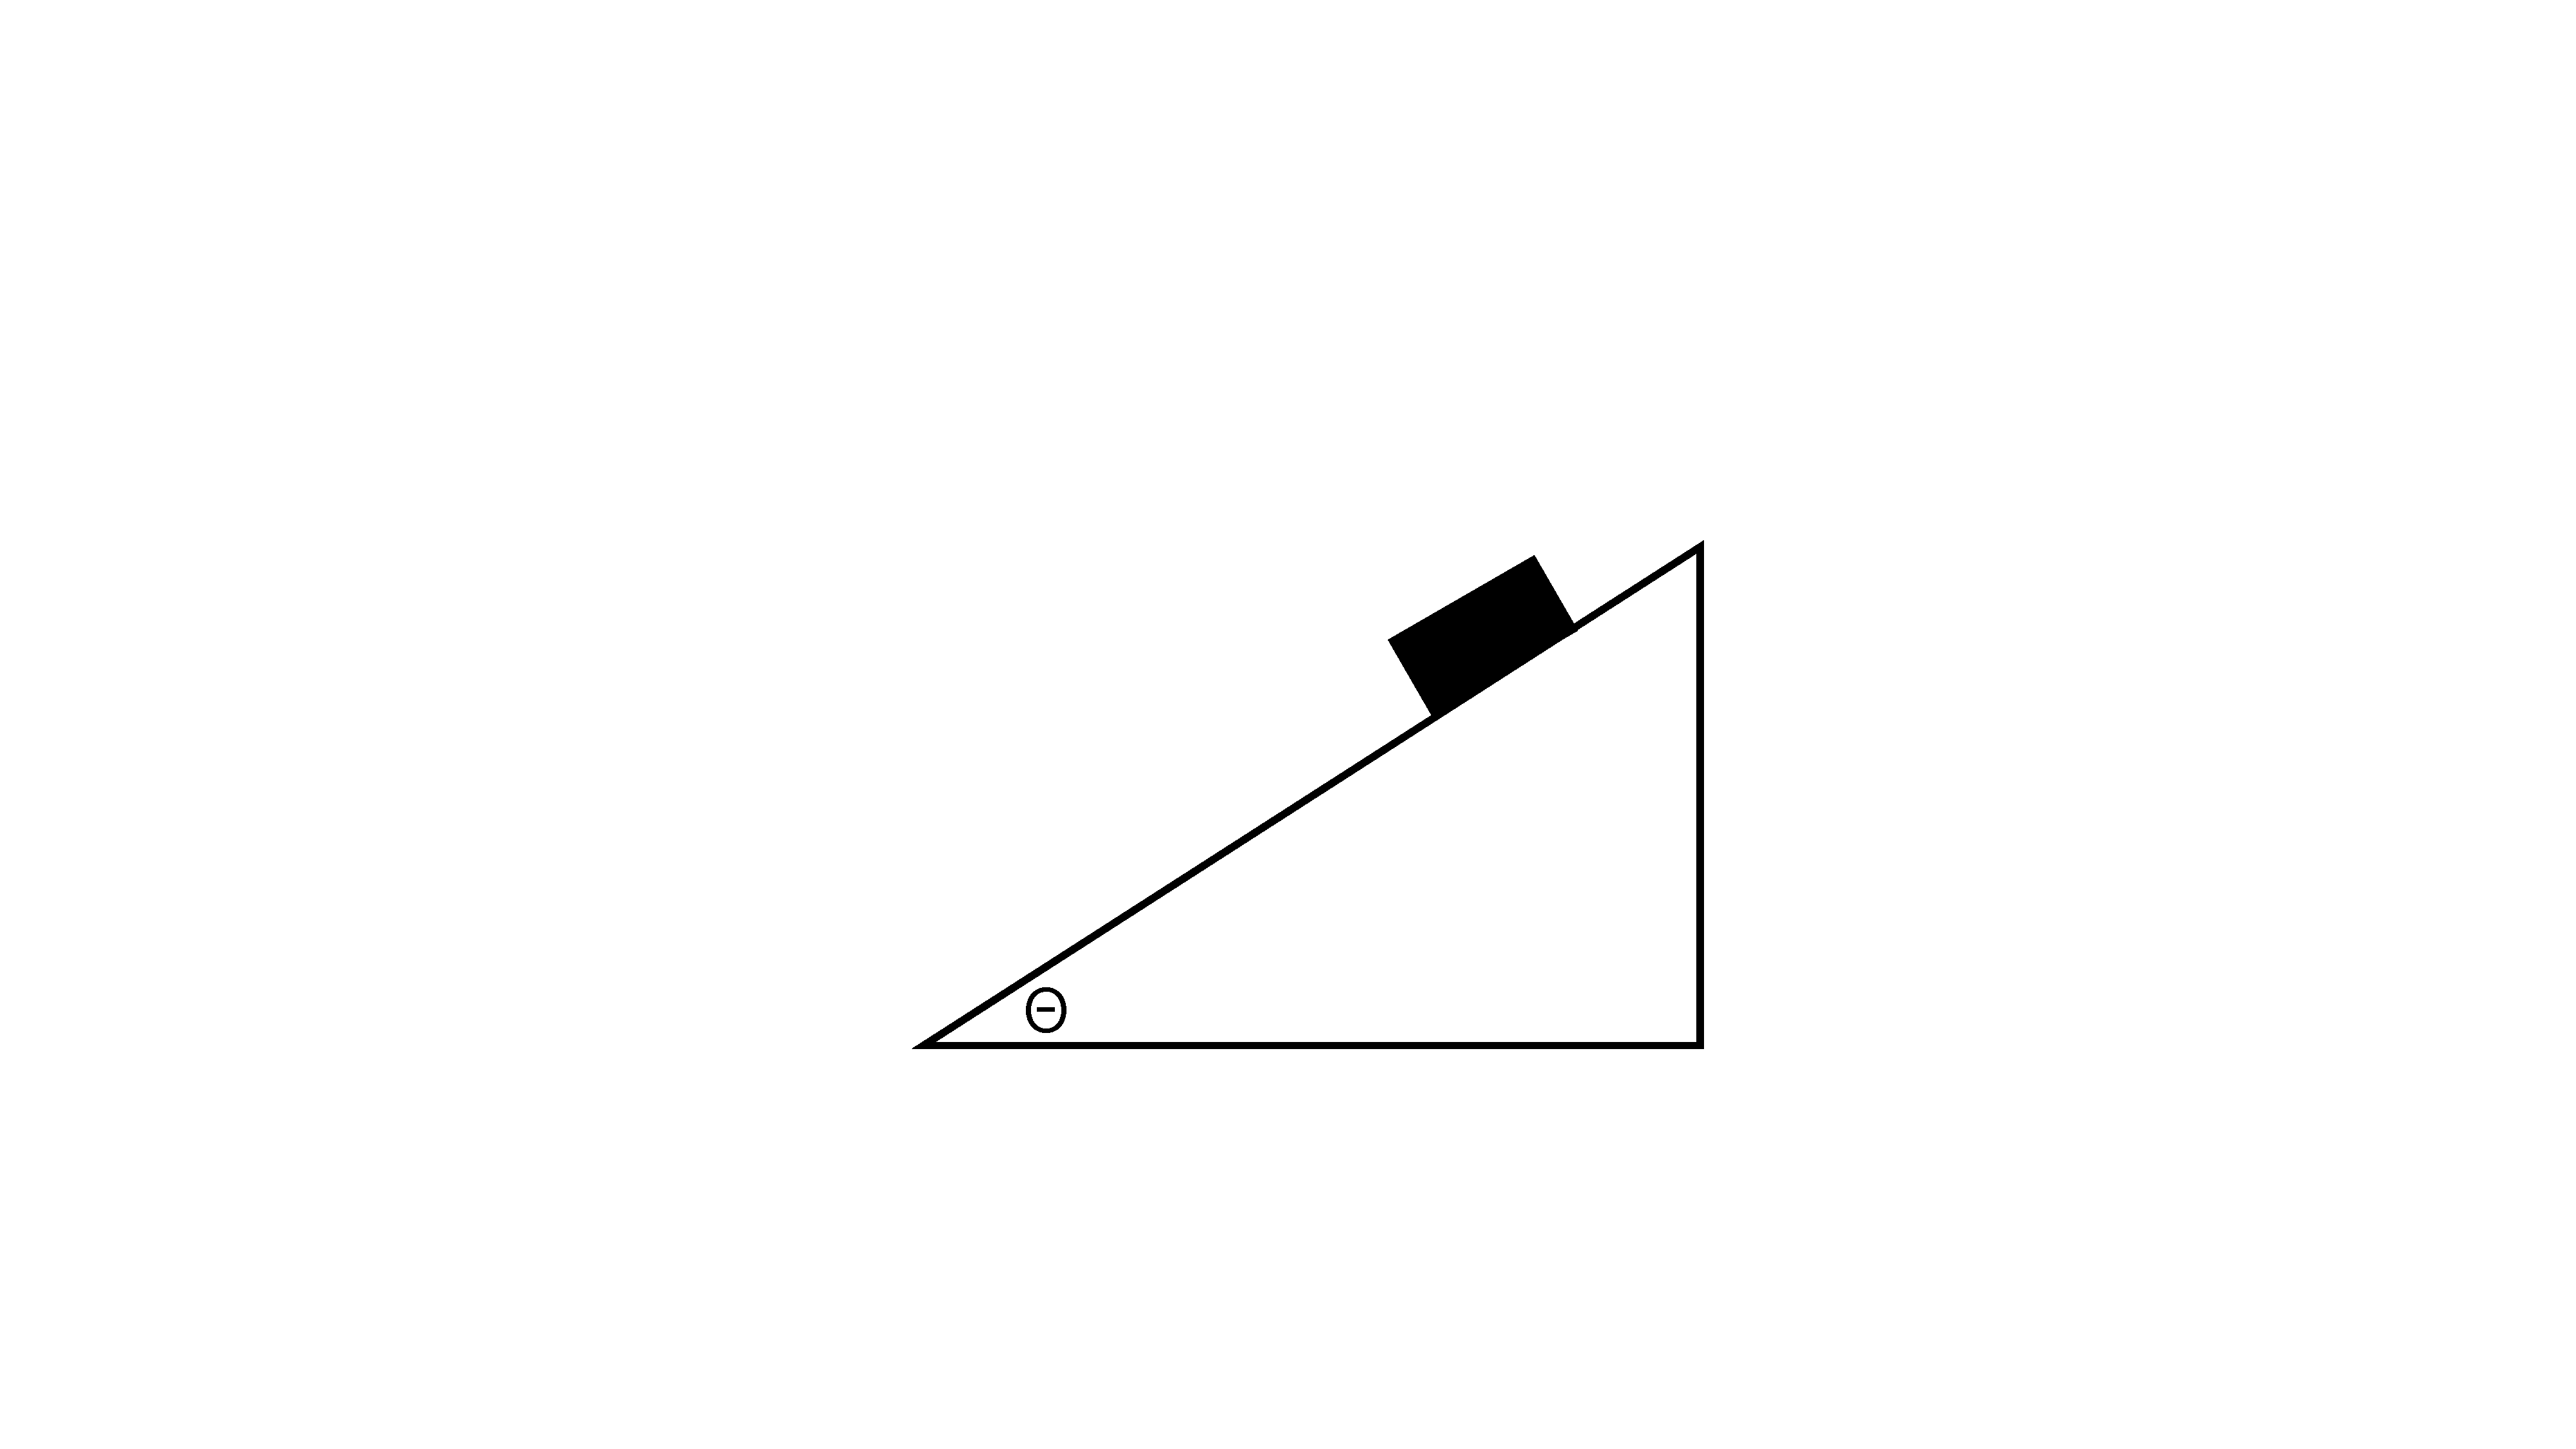
\includegraphics[width=5cm]{friction_ramp.pdf}
\end{center}
\begin{parts}
	\part[5] Draw a free body diagram representing the forces acting on the block (be sure to label the object in the surrounding which is exerting the force)
	\vspace{5cm}
	\part[15] What is the coefficient of kinetic friction $\mu$ between the block and the ramp?
\end{parts}